\documentclass[aspectratio=169]{beamer}

% Tema e Cores
\usetheme{Madrid}   % Temas: Boadilla, CambridgeUS, metropolis, Madrid, Frankfurt
\usecolortheme{spruce} % seahorse, spruce

% Pacotes de Idioma e Codificação
\usepackage[utf8]{inputenc}
\usepackage[brazilian]{babel}
\usepackage[T1]{fontenc}

% Pacotes Gráficos e de Tabelas
\usepackage{graphicx}
\usepackage{booktabs}
\usepackage{multirow}
\usepackage{tikz}
\usepackage{qrcode}


% --- COMANDO PARA INSERIR A LOGO ANTES DO TÍTULO ---
\addtobeamertemplate{title page}{
    \centering
    
\includegraphics[height=2.7cm]{logo-erin2.png}\par
}{}

% Informações da Capa
\title[Modelos Preditivos para Empréstimos]{Modelos Preditivos para Estimação de Status de Empréstimos Bancários via Machine Learning: Uma Abordagem Baseada na Metodologia CRISP-DM}

\author[Valente, Silva \& Morais]{Mário Diego Valente\inst{1} \and Gabriel Baia da Silva\inst{1} \and Jefferson Magalhães de Morais\inst{2}}

\institute[UFPA]{
  \inst{1} Graduando em Sistemas de Informação - UFPA\\
  \inst{2} Professor Dr., Faculdade de Computação - UFPA
}


\begin{document}

%==============================================================================%
% --- SLIDE 1: Capa ---
\begin{frame}
    \titlepage
\end{frame}
%==============================================================================%

%==============================================================================%
% --- SLIDE 2: Introdução ---
\begin{frame}{Introdução e Objetivos}
    \textbf{Contexto}
    \begin{itemize}
        \item A análise de solicitações de crédito imobiliário exige equilíbrio entre \textbf{eficiência operacional} e \textbf{capacidade de discriminação}.
        \item Modelos preditivos auxiliam na triagem de propostas utilizando características cadastrais, financeiras e imobiliárias.
    \end{itemize}
    \vspace{0.5cm}
    
    \textbf{Objetivo do Trabalho}
    \begin{itemize}
        \item Aplicar modelos preditivos de \textit{Machine Learning} para classificação do status de aprovação de empréstimos.
        \item Comparar oito classificadores e identificar o mais adequado utilizando a metodologia \textbf{CRISP-DM}.
    \end{itemize}
\end{frame}
%==============================================================================%

%==============================================================================%
%==============================================================================%
% --- SLIDE 3: Base de Dados e Preparação ---
\begin{frame}{Metodologia: Dados e Preparação}
    \textbf{Entendimento dos Dados}
    \begin{itemize}
        \item \textbf{Dataset:} \texttt{loan\_data.csv} (Kaggle / Disponível em: \href{https://github.com/MarioDhiego/Slide_ERIN_2026/blob/main/loan_data.csv}{\color{blue}\underline{GitHub do Projeto}}).
        \item \textbf{Tamanho:} 381 registros e 13 variáveis.
        \item \textbf{Variável-alvo:} \texttt{Loan\_Status} (0 = Reprovado; 1 = Aprovado).
    \end{itemize}
    \vspace{0.3cm}
    
    \textbf{Preparação da Base}
    \begin{itemize}
        \item Tratamento de valores ausentes (moda para categóricas e mediana para numéricas).
        \item Transformação por \textit{Label Encoding}.
        \item \textbf{Divisão da Amostra:} 80\% Treino e 20\% Teste.
        \item Aplicação de padronização escalar rigorosa (Z-score).
    \end{itemize}
\end{frame}
%==============================================================================%
%==============================================================================%

%==============================================================================%
% --- SLIDE 4: Ferramentas ---
\begin{frame}{Metodologia: Ferramentas Utilizadas}
Para conduzir as análises e estimativas neste estudo, foi adotada a linguagem de programação \textbf{Python}, utilizando a IDE \href{https://colab.research.google.com/drive/1bM0SFVu0IQhGwztcZHo2HhptDlSos2jZ#scrollTo=lNeeCTE95Ab9}{\color{blue}\textbf{\underline{Google Colaboratory}}} na versão 3.10.12. Foram empregadas as seguintes bibliotecas para implementação das diversas etapas do processo:  
    \vspace{0.3cm}
    \begin{itemize}
        \item NumPy [OLIPHANT, T. E. et al. (2006)]
        \item Pandas [MCKINNEY, W. (2010)]
        \item Matplotlib [HUNTER, J. D. (2007)]
        \item Seaborn [WASKOM, M. (2021)]
        \item Scikit-learn [PEDREGOSA, F. et al. (2011)]
    \end{itemize}
\end{frame}
%==============================================================================%

%==============================================================================%
% --- SLIDE 5: Modelagem ---
\begin{frame}{Metodologia: Modelagem e Avaliação}
    \textbf{Modelos Avaliados (8 classificadores)}
    \begin{itemize}
        \item Regressão Logística (\textit{baseline})
        \item Árvore de Decisão e Random Forest
        \item k-Nearest Neighbors (kNN)
        \item Naive Bayes Gaussiano (NBG)
        \item Support Vector Machine (SVM)
        \item Multilayer Perceptron (MLP)
      %  \item Voting Classifier (\textit{soft voting})
    \end{itemize}
    \vspace{0.3cm}
    
    \textbf{Otimização e Validação}
    \begin{itemize}
        \item \textit{Grid Search} associado à \textbf{Validação Cruzada 10-fold}.
        \item Métricas: Acurácia, Precisão, Revocação, F1-Score, AUC, Gini e KS.
    \end{itemize}
\end{frame}
%==============================================================================%

%==============================================================================%
% --- SLIDE 6: Métricas Parte 1 ---
\begin{frame}{Métricas de Avaliação I}
    O desempenho dos modelos foi inicialmente mensurado com base nos Verdadeiros Positivos (VP), Verdadeiros Negativos (VN), Falsos Positivos (FP) e Falsos Negativos (FN).
    
    \vspace{0.2cm}
    \begin{itemize}
        \item \textbf{Acurácia (Acc):} Taxa global de acertos do modelo.
        $ Acc = \frac{VP + VN}{VP + VN + FP + FN} $
        
        \vspace{0.1cm}
        \item \textbf{Precisão (Precision):} Foco na exatidão das predições positivas.
        $ Prec = \frac{VP}{VP + FP} $
        
        \vspace{0.1cm}
        \item \textbf{Revocação (Recall/Sensibilidade):} Capacidade de detectar os positivos reais.
        $ Rec = \frac{VP}{VP + FN} $
        
        \vspace{0.1cm}
        \item \textbf{F1-Score:} Média harmônica entre Precisão e Revocação (robusta ao desbalanceamento).
        $ F1 = 2 \cdot \frac{Prec \cdot Rec}{Prec + Rec} $
    \end{itemize}
    
    \vfill
    \hrule
    \vspace{0.1cm}
    {\tiny \textbf{Fundamentação:} THARWAT, A. Classification assessment methods. \textit{Applied Computing and Informatics}, v. 17, n. 1, p. 168-192, 2021.}
\end{frame}
%==============================================================================%

%==============================================================================%
% --- SLIDE 7: Métricas Parte 2 ---
\begin{frame}{Métricas de Avaliação II}
    Para avaliar a capacidade do modelo em \textbf{separar e ordenar} os perfis de risco (bom vs. mau pagador), empregaram-se métricas baseadas em limiares e probabilidade:
    
    \vspace{0.2cm}
    \begin{itemize}
        \item \textbf{AUC-ROC (Area Under the Curve):} Mede a distinção entre as classes em vários limiares (Integra a Taxa de VP pela Taxa de FP).
        $$ AUC = \int_{0}^{1} TPR(t) \, d(FPR(t)) $$
        
        \item \textbf{Índice de Gini:} Derivado da AUC, quantifica o poder discriminatório geral.
        $$ Gini = 2 \cdot AUC - 1 $$
        
        \item \textbf{Estatística KS (Kolmogorov-Smirnov):} Mede a distância máxima entre as funções de distribuição acumulada dos aprovados ($F_{pos}$) e reprovados ($F_{neg}$).
        $$ KS = \max_{c} |F_{pos}(c) - F_{neg}(c)| $$
    \end{itemize}
    
    \vfill
    \hrule
    \vspace{0.1cm}
    {\tiny \textbf{Fundamentação:} GRANDINI, M.; BAGLI, E.; VISANI, G. Metrics for Multi-Class Classification: an Overview. \textit{arXiv:2008.05756}, 2020.}
\end{frame}
%==============================================================================%

%==============================================================================%
% --- SLIDE 8: Resultados - Exploratória Numérica ---
\begin{frame}{Resultados: Análise Exploratória de Dados (1/2)}
A fim de compreender as características intrínsecas da base, estatísticas descritivas foram extraídas. A Tabela \ref{tab:1} apresenta um resumo dos atributos numéricos (em sua escala original para facilitar a interpretação).

\begin{table}[htbp]
    \centering
    \caption{Estatísticas dos atributos numéricos.}
    {\small
    \begin{tabular}{l|c|c|c|c} 
          \hline \hline
        \textbf{Variável} & \textbf{Média} & \textbf{Desv. Pad.}   & \textbf{Min} & \textbf{Max} \\ 
          \hline \hline
        Renda do Candidato                 & \$ 3.579,85 & \$ 1.419,81  & \$ 150,00     & \$ 9.703,00 \\
        Renda do Fiador                    & \$ 1.277,28 & \$ 2.340,82  & \$ 0,00       & \$ 33.837,00 \\
        Valor Empréstimo (milhares)        & \$ 104.986   & \$ 28.358   & \$ 9.000,00   & 150.000,00 \\
        Prazo do Empréstimo (meses)        & 341          &  68         & 12            & 480 \\
          \hline \hline
    \end{tabular}
    }
    \label{tab:1}
\end{table}
\end{frame}
%==============================================================================%

%==============================================================================%
% --- SLIDE 9: Resultados - Exploratória Categórica ---
\begin{frame}{Resultados: Análise Exploratória de Dados (2/2)}
\begin{table}[htbp]
    \centering
    \caption{Distribuição dos Atributos Categóricos.}
    \begin{tabular}{l|c|c|c} 
          \hline \hline
        \textbf{Atributo}     & \textbf{Moda} & \textbf{Frequência} & \textbf{Relativa (\%)} \\ 
          \hline \hline
        Gênero                & Masculino     & 296                 & 77,69 \\
        Estado Civil          & Casado        & 228                 & 59,84 \\
        Nº de Dependentes     & 1             & 242                 & 63,52 \\
        Escolaridade          & Graduação     & 278                 & 72,97 \\
        Trabalhador Autônomo  & Não           & 346                 & 90,81 \\
        Histórico de Crédito  & Sim           & 324                 & 85,04 \\
        Área de Residência    & Semiurbana    & 149                 & 39,11 \\
        Status de Empréstimo  & Aprovado      & 271                 & 71,13 \\ 
          \hline \hline
    \end{tabular} 
    \label{tab:2}
\end{table}
\end{frame}
%==============================================================================%

%==============================================================================%
% --- SLIDE 10: Resultados - Tabela de Desempenho ---
\begin{frame}{Resultados: Desempenho Geral dos Modelos}
    \begin{table}[]
        \centering
        \caption{Avaliação dos modelos no conjunto de teste.}
        \vspace{0.1cm}
        \resizebox{\textwidth}{!}{
        \begin{tabular}{l|c|c|c|c|c}
              \hline \hline
            \textbf{Modelo} & \textbf{Acurácia (\%)} & \textbf{F1-Score (\%)} & \textbf{AUC (\%)} & \textbf{Gini (\%)} & \textbf{KS (\%)} \\ 
              \hline \hline
            \textbf{Random Forest} & \textbf{85,7} & \textbf{90,8} & \textbf{82,6} & \textbf{65,3} & 54,5 \\
            Regressão Logística & \textbf{85,7} & \textbf{90,8} & 72,7 & 45,5 & 54,5 \\
            Naive Bayes & \textbf{85,7} & \textbf{90,8} & 70,1 & 40,2 & 52,7 \\
            Árvore de Decisão & 75,3 & 82,9 & 69,1 & 38,2 & 43,6 \\
            MLP & 68,8 & 81,0 & 54,7 & 9,4 & 21,8 \\
            kNN & 68,8 & 79,7 & 48,1 & -3,7 & 16,4 \\
            SVM & 71,4 & 83,3 & 44,0 & -11,9 & 25,5 \\ 
              \hline \hline
        \end{tabular}
        }
    \end{table}
    \small{\textit{Nota:} Random Forest obteve o maior poder discriminatório isolado (AUC e Gini).}
\end{frame}
%==============================================================================%

%==============================================================================%
% --- SLIDE 11: Curva ROC ---
\begin{frame}{Resultados: Análise da Curva ROC}
    \begin{columns} 
        \column{0.62\textwidth}
        \begin{figure}
            \centering
            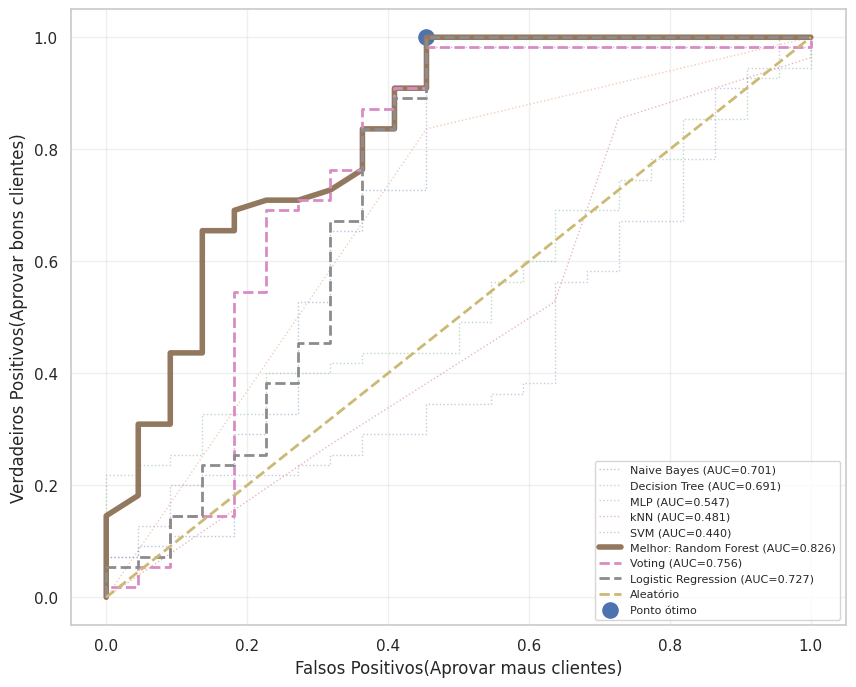
\includegraphics[width=0.95\textwidth]{curva_roc_geral.png}
        \end{figure}
    \end{columns}
\end{frame}
%==============================================================================%

%==============================================================================%
% --- SLIDE 12: Teste de DeLong ---
\begin{frame}{Resultados: Teste Estatístico de DeLong}
    \begin{itemize}
        \item O \textbf{Teste de DeLong} foi aplicado para verificar a \textbf{significância estatística} das diferenças empíricas entre as áreas sob a curva (AUC).
        \item \textbf{Random Forest (Baseline):} Possui diferença significativa em relação à maioria dos modelos, \textbf{exceto} para Regressão Logística.
    \end{itemize}
    \vspace{0.2cm}
    
    \begin{table}
        \centering
        \caption{Comparação com o modelo de melhor desempenho (Random Forest)}
        \vspace{0.1cm}
        \resizebox{0.70\textwidth}{!}{
        \begin{tabular}{l|c|c}
            \hline \hline
            \textbf{Modelo Avaliado} & \textbf{Valor-p} & \textbf{Dif. Significativa ($\alpha = 0{,}05$)} \\  \hline \hline
         %   Voting & $0{,}112310$ & Não \\
            Regressão Logística & $0{,}100014$ & Não \\
            Naive Bayes & $< 0{,}006914$ & Sim \\
            Árvore de Decisão & $< 0{,}018508$ & Sim \\
            MLP & $< 0{,}000410$ & Sim \\
            SVM & $< 0{,}000718$ & Sim \\
            kNN & $< 0{,}000041$ & Sim \\ 
             \hline \hline
        \end{tabular}
        }
    \end{table}
\end{frame}
%==============================================================================%

%==============================================================================%
% --- SLIDE 13: Análise do Modelo Definitivo ---
\begin{frame}{Resultados: O Modelo Definitivo (Random Forest)}
    \begin{columns}
        \column{0.48\textwidth}
        \textbf{Matriz de Confusão (77 instâncias)}
        \begin{itemize}
            \item \textbf{Verdadeiros Positivos (54):} Bons pagadores aprovados corretamente.
            \item \textbf{Verdadeiros Negativos (12):} Maus pagadores identificados e negados.
            \item \textbf{Falsos Negativos (1):} Apenas um bom cliente negado (praticamente não há perda de bons negócios).
            \item \textbf{Falsos Positivos (10):} Risco de calote sob rígido controle.
        \end{itemize}
        
        \column{0.50\textwidth}
        \textbf{Métricas de Risco e Negócio}
        \begin{itemize}
            \item \textbf{Recall (98,1\%):} Praticamente perfeito. Garante que os clientes lucrativos não sejam afugentados pela instituição.
            \item \textbf{Gini (65,3\%):} No mercado financeiro, valores superiores a 60\% indicam um modelo fortíssimo e lucrativo.
            \item \textbf{KS (54,5\%):} Separação formidável. A distância entre bons e maus clientes ultrapassa 50\%, provando uma segmentação altamente eficaz.
        \end{itemize}
    \end{columns}
\end{frame}
%==============================================================================%

%==============================================================================%
% --- SLIDE 14: Considerações Finais ---
\begin{frame}{Considerações Finais e Trabalhos Futuros}
    \textbf{Conclusões}
    \begin{itemize}
        \item O \textbf{Random Forest} apresentou o melhor desempenho descritivo e a maior capacidade discriminatória global no cenário estudado.
        \item O modelo demonstrou-se apto para \textbf{minimizar falsos positivos}, protegendo a instituição de perdas diretas sem penalizar erroneamente bons pagadores.
    \end{itemize}
    \vspace{0.5cm}
    
    \textbf{Trabalhos Futuros}
    \begin{itemize}
        \item Aplicação de técnicas de balanceamento amostral sintético prévio (Ex: SMOTE).
        \item Estudo de explicabilidade do modelo (\textit{eXplainable AI} via SHAP) para adequação às exigências e regulações financeiras de transparência.
    \end{itemize}
\end{frame}
%==============================================================================%


%==============================================================================%
% --- SLIDES DE REFERÊNCIAS BIBLIOGRÁFICAS ---
\begin{frame}[allowframebreaks]{Referências Bibliográficas}
    \scriptsize % Reduz o tamanho da fonte para caber mais referências
    \begin{thebibliography}{99}

    \bibitem{maciel2015}
    MACIEL, H. M.; MACIEL, W. M. 
    \newblock Análise da inadimplência em uma instituição financeira na região metropolitana de Fortaleza.
    \newblock \emph{Essentia - Revista de Cultura, Ciência e Tecnologia da UVA}, v. 16, n. 2, 2015.

    \bibitem{morettin2022}
    MORETTIN, P. A.; SINGER, J. M.
    \newblock \emph{Estatística e ciência de dados}.
    \newblock Rio de Janeiro: LTC, 2022. 454 p.

    \bibitem{morais2024}
    MORAIS, J. M.
    \newblock CRISP-DM: A metodologia certa para projetos de machine learning.
    \newblock Material didático da disciplina Tópicos Especiais em AM, Faculdade de Computação, UFPA, 2024.

    \bibitem{monard2003}
    MONARD, M. C.; BARANAUSKAS, J. A.
    \newblock Conceitos sobre aprendizado de máquina.
    \newblock \emph{Sistemas Inteligentes - Fundamentos e aplicações}, 2003.

    \bibitem{izbicki2020}
    IZBICKI, R.; SANTOS, T. M. dos.
    \newblock \emph{Aprendizado de máquina: uma abordagem estatística}.
    \newblock 1. ed. 2020.

    \bibitem{chapman2000}
    CHAPMAN, P. et al.
    \newblock CRISP-DM 1.0: Step-by-step data mining guide.
    \newblock \emph{SPSS Inc.}, 2000.

    \bibitem{numpy2020}
    HARRIS, C. R. et al.
    \newblock Array programming with NumPy.
    \newblock \emph{Nature}, v. 585, n. 7825, p. 357–362, 2020.

    \bibitem{pandas2020}
    THE PANDAS DEVELOPMENT TEAM.
    \newblock pandas-dev/pandas: Pandas, 2020.

    \bibitem{mckinney2010}
    MCKINNEY, W.
    \newblock Data Structures for Statistical Computing in Python.
    \newblock In: \emph{Proceedings of the 9th Python in Science Conference}, p. 56–61, 2010.

    \bibitem{matplotlib2007}
    HUNTER, J. D.
    \newblock Matplotlib: A 2D graphics environment.
    \newblock \emph{Computing in Science \& Engineering}, v. 9, n. 3, p. 90–95, 2007.

    \bibitem{seaborn2021}
    WASKOM, M. L.
    \newblock seaborn: statistical data visualization.
    \newblock \emph{Journal of Open Source Software}, v. 6, n. 60, p. 3021, 2021.

    \bibitem{scikit2011}
    PEDREGOSA, F. et al.
    \newblock Scikit-learn: Machine learning in Python.
    \newblock \emph{Journal of Machine Learning Research}, v. 12, p. 2825–2830, 2011.

    \bibitem{scikit2013}
    BUITINCK, L. et al.
    \newblock API design for machine learning software: experiences from the scikit-learn project.
    \newblock In: \emph{ECML PKDD Workshop}, p. 108–122, 2013.

    \end{thebibliography}
\end{frame}
%==============================================================================%



%==============================================================================%
% --- SLIDE 15: Encerramento ---
\begin{frame}
    \centering
    \Huge \textbf{Obrigado!}
    
    \vspace{0.5cm}
    
    \qrcode[height=3.5cm]{https://github.com/MarioDhiego/Slide_ERIN_2026/blob/main/Artigo_Slide_ERIN_2026.pdf}
    
    \vspace{1cm}
    
    % --- Contatos um embaixo do outro ---
    \normalsize
    \textbf{Contatos:}\\
    diego.valente@gmail.com\\
    gabrielkadran@hotmail.com\\
    jmorais@ufpa.br
\end{frame}
%==============================================================================%







\end{document}